%!TeX program = xelatex
\documentclass[12pt,a4paper,UTF8]{ctexart}
\usepackage{zjureport-main/zjureport}

\setcounter{tocdepth}{2}
\captionsetup{font=small,skip=3pt}
\setlength{\textfloatsep}{8pt plus 2pt minus 2pt}
\setlength{\floatsep}{6pt plus 2pt minus 2pt}
\setlength{\intextsep}{6pt plus 2pt minus 2pt}
\setlength{\abovedisplayskip}{6pt plus 2pt minus 2pt}
\setlength{\belowdisplayskip}{6pt plus 2pt minus 2pt}
\setlength{\abovedisplayshortskip}{4pt plus 2pt minus 2pt}
\setlength{\belowdisplayshortskip}{4pt plus 2pt minus 2pt}

\lstdefinestyle{codestyle}{
  basicstyle=\ttfamily\small,
  keywordstyle=\color{blue!65!black},
  commentstyle=\color{green!40!black},
  stringstyle=\color{orange!70!black},
  breaklines=true,
  frame=single,
  columns=fullflexible,
  keepspaces=true,
  showstringspaces=false
}
\lstset{style=codestyle}

\graphicspath{{./}{images/}{zjureport-main/figures/}{../outputs/figures/}}

\newcommand{\figplaceholder}[2]{
  \begin{figure}[H]
    \centering
    \IfFileExists{#1}{
      \includegraphics[width=0.88\linewidth]{#1}
    }{
      \fbox{\parbox[c][5.0cm][c]{0.82\linewidth}{\centering
      图像文件尚未生成：\\ \path{#1}\\[0.5em]
      可运行 \texttt{python main.py --n 3 --target 101 --iterations 2} 生成。}}
    }
    \caption{#2}
  \end{figure}
}

\title{
  \vspace{3cm}
  \heiti \Huge \textbf{量子计算课程报告}\par
  \vspace{1cm}
  \heiti \Large Grover搜索算法可视化演示系统
  \vspace{3cm}
}
\author{
  \vspace{0.5cm}
  \kaishu\Large 姓名\ \dlmu[9cm]{} \qquad \\
  \vspace{0.5cm}
  \kaishu\Large 学号\ \dlmu[9cm]{} \qquad \\
  \vspace{0.5cm}
  \kaishu\Large 院所\ \dlmu[9cm]{}
}
\date{\today}

\begin{document}

\cover
\thispagestyle{empty}

\newpage
\tableofcontents

\newpage

\begin{abstract}
本课程项目围绕“Grover搜索算法中振幅放大过程的步进式3D展示”展开，搭建了一个支持2到3个量子比特的Grover算法玩具模型。项目重点不是求解大规模搜索问题，而是把抽象的量子态演化拆解为可观察的中间步骤：Hadamard门制备均匀叠加态，Oracle对目标态执行相位翻转，Diffusion算子执行关于平均概率幅的反演，并在每一步后保存statevector。实现上，项目使用Qiskit构造量子电路和提取中间态，使用Streamlit构建交互界面，使用Plotly绘制概率幅柱状图、概率柱状图、目标态概率曲线以及可旋转缩放的3D步进概率历史图。实验结果表明，在3量子比特、目标态为\(|101\rangle\)的例子中，目标态概率由初始的\(12.5\%\)经一次完整Grover迭代提升至\(78.125\%\)，两次迭代后提升至\(94.53125\%\)，直观体现了Grover算法的振幅放大机制。
\end{abstract}

\textbf{关键词：} Grover搜索；振幅放大；Oracle；均值倒置；Qiskit；Streamlit；Plotly；3D可视化

\section{项目背景与目标}

Grover搜索算法是量子计算中最具代表性的算法之一。对于含有\(N=2^n\)个候选状态、且只有一个目标解的无结构搜索问题，经典穷举搜索平均需要\(O(N)\)次查询，而Grover算法只需要约\(O(\sqrt{N})\)次Oracle查询即可显著提高目标态被测得的概率。

从应用角度看，Grover算法并不只对应“在数据库里找一条记录”这一种直观场景。更一般地，只要一个问题可以被表述为“在大量候选解中寻找满足判定条件的解”，就可以把判定条件封装为Oracle，再利用Grover式振幅放大提高正确候选被测量到的概率。典型应用包括：无结构数据库或索引检索、密码学中的密钥搜索与哈希原像搜索、组合优化中的可行解搜索、约束满足问题中的候选筛选，以及作为其他量子算法子程序的幅度放大模块。虽然真实应用还需要考虑Oracle构造成本、硬件噪声和量子资源开销，但Grover算法提供的平方级加速仍然是理解量子搜索优势的重要入口。

不过，对于初学者而言，Grover算法的难点往往不在最终测量结果，而在于理解“振幅放大”到底如何发生。Oracle本身并不会直接增加目标态概率，它只是把目标态的概率幅乘以\(-1\)，也就是完成相位标记。真正把相位标记转化为概率提升的是Diffusion算子，即关于平均概率幅的反演。

因此，本项目的目标设定为：
\begin{enumerate}
  \item 构造一个支持2到3个量子比特的Grover搜索玩具模型；
  \item 支持任意计算基目标态，例如\(|10\rangle\)、\(|101\rangle\)；
  \item 在Hadamard初始化、每次Oracle操作、每次Diffusion操作后保存中间statevector；
  \item 用2D柱状图和3D步进图展示各基态概率幅和概率的变化；
  \item 通过交互式滑块、动画和电路视图帮助观察“Oracle翻转”和“均值倒置”的作用差异。
\end{enumerate}

\section{Grover算法原理}

\subsection{问题模型}

设搜索空间大小为
\[
N=2^n,
\]
其中\(n\)为量子比特数。目标态记为\(|\omega\rangle\)。初始状态\(|0\rangle^{\otimes n}\)经过Hadamard门后变为均匀叠加态：
\[
|s\rangle = H^{\otimes n}|0\rangle^{\otimes n}
= \frac{1}{\sqrt{N}}\sum_{x=0}^{N-1}|x\rangle.
\]

对于单目标搜索，目标态的初始测量概率为
\[
P_0=\left|\frac{1}{\sqrt{N}}\right|^2=\frac{1}{N}.
\]
当\(n=3\)时，\(N=8\)，因此目标态初始概率只有\(12.5\%\)。

\subsection{Oracle相位翻转}

Oracle的作用是识别目标态，并只改变目标态的相位：
\[
O|\omega\rangle=-|\omega\rangle,\qquad O|x\rangle=|x\rangle\quad(x\ne \omega).
\]

因此，Oracle后目标态概率幅的符号发生翻转，但概率
\[
P_\omega = |a_\omega|^2
\]
不会因为单纯的符号改变而上升。这一点是本项目可视化的重点之一：在概率幅图中可以看到目标态柱子翻到零轴下方，而在概率图中目标态柱子的高度暂时不变。

\subsection{Diffusion均值倒置}

Diffusion算子可写为
\[
D=2|s\rangle\langle s|-I.
\]
从概率幅角度看，它等价于把每个概率幅\(a_i\)关于平均概率幅\(\bar{a}\)做反演：
\[
a_i' = 2\bar{a}-a_i,\qquad
\bar{a}=\frac{1}{N}\sum_{i=0}^{N-1}a_i.
\]

Oracle把目标态振幅翻成负值后，会改变全体振幅的平均值。Diffusion再对所有振幅做均值倒置，于是目标态振幅从负值被反演到较大的正值，非目标态振幅则被压低。这样，相位信息被转化为测量概率的提升。

\subsection{理论概率公式}

令
\[
\sin\theta=\frac{1}{\sqrt{N}}.
\]
完成\(r\)次完整Grover迭代后，目标态理论概率为
\[
P_r=\sin^2((2r+1)\theta).
\]
最佳迭代次数近似为
\[
r^\ast \approx \left\lfloor \frac{\pi}{4}\sqrt{N}\right\rceil.
\]
由于本项目只展示2到3个量子比特，搜索空间很小，目标态概率会在少数几次迭代内迅速升高，继续迭代还会出现“过迭代”导致概率回落的现象。

\section{系统设计}

\subsection{项目结构}

本项目代码结构如下：

\begin{lstlisting}[language=bash]
grover_qiskit_ui_refined/
|-- app.py                    # Streamlit交互界面
|-- main.py                   # 命令行图片和CSV导出入口
|-- qiskit_grover_core.py     # Grover电路构造与statevector分析
|-- visualization.py          # Matplotlib/Plotly可视化函数
|-- requirements.txt          # Python依赖
`-- README.md                 # 项目说明
\end{lstlisting}

其中，\texttt{qiskit\_grover\_core.py}负责算法和量子态演化，\texttt{visualization.py}负责图形绘制，\texttt{app.py}负责交互界面组织，\texttt{main.py}用于离线生成报告图片和CSV数据。

\subsection{技术选型}

项目采用的主要技术如下：

\begin{table}[H]
\centering
\caption{项目技术选型}
\begin{tabular}{lll}
\toprule
模块 & 工具 & 作用 \\
\midrule
量子电路 & Qiskit & 构造Hadamard、Oracle、Diffusion和测量电路 \\
中间态分析 & Statevector & 提取每一步后的精确量子态 \\
静态绘图 & Matplotlib & 导出概率幅图、概率图和标准电路图 \\
交互绘图 & Plotly & 绘制交互式柱状图、3D概率历史图和动画 \\
网页界面 & Streamlit & 提供参数选择、滑块和图表展示 \\
可选仿真 & Qiskit Aer & 进行shots测量统计和简化噪声对照 \\
\bottomrule
\end{tabular}
\end{table}

\subsection{步进式历史状态设计}

为了展示每一步的变化，程序没有只保存最终电路，而是定义了\texttt{GroverStep}数据结构，用于记录每一个中间阶段：
\begin{itemize}
  \item \texttt{index}：步骤编号；
  \item \texttt{kind}：步骤类型，包括\texttt{initial}、\texttt{oracle}、\texttt{diffusion}；
  \item \texttt{iteration}：当前属于第几轮Grover迭代；
  \item \texttt{circuit}：当前量子电路副本；
  \item \texttt{statevector}：当前电路对应的精确量子态。
\end{itemize}

核心流程为：
\begin{enumerate}
  \item 对所有量子比特施加Hadamard门，保存初始均匀叠加态；
  \item 每轮迭代先施加Oracle，保存Oracle相位翻转后的statevector；
  \item 再施加Diffusion，保存均值倒置后的statevector；
  \item 将所有步骤传给可视化模块，绘制逐步演化图。
\end{enumerate}

\subsection{关键实现方法}

\subsubsection{多控制相位翻转}

Oracle和Diffusion都需要对\(|11\cdots 1\rangle\)执行相位翻转。程序将这个操作封装为\texttt{\_apply\_multi\_controlled\_z}。当量子比特数为1时直接使用\(Z\)门；当量子比特数大于1时，程序用\(H-\mathrm{MCX}-H\)把多控制\(X\)门转化为多控制\(Z\)门：

\begin{lstlisting}[language=Python]
def _apply_multi_controlled_z(qc, qubits):
    if len(qubits) == 1:
        qc.z(qubits[0])
        return

    controls = qubits[:-1]
    target = qubits[-1]
    qc.h(target)
    qc.mcx(controls, target)
    qc.h(target)
\end{lstlisting}

以3量子比特为例，该函数会对\(|111\rangle\)态乘以\(-1\)，其余计算基态保持不变。

\subsubsection{目标态Oracle构造}

项目允许用户选择任意目标态。Oracle的目标是只对该目标态执行相位翻转。实现时，程序先把目标态临时映射到\(|11\cdots 1\rangle\)，再调用多控制相位翻转，最后恢复原来的计算基顺序。

例如目标态为\(|101\rangle\)时，中间的第2位为0，程序会先对对应量子比特施加\(X\)门，把\(|101\rangle\)映射到\(|111\rangle\)。完成多控制\(Z\)门后，再施加一次\(X\)门还原：

\begin{lstlisting}[language=Python]
def apply_oracle(qc, target, add_barrier=True):
    n = len(target)

    for qubit, bit in enumerate(target):
        if bit == "0":
            qc.x(qubit)

    _apply_multi_controlled_z(qc, list(range(n)))

    for qubit, bit in enumerate(target):
        if bit == "0":
            qc.x(qubit)

    if add_barrier:
        qc.barrier()
\end{lstlisting}

因此，对于任意用户输入的目标比特串，Oracle都会实现
\[
O|\omega\rangle=-|\omega\rangle,\qquad O|x\rangle=|x\rangle\quad(x\ne \omega).
\]

\subsubsection{Diffusion算子构造}

Diffusion算子采用标准的\(H-X-\mathrm{MCZ}-X-H\)结构。程序先用Hadamard门和\(X\)门把关于均匀叠加态的反演转换为对\(|11\cdots 1\rangle\)的相位翻转，再恢复基底：

\begin{lstlisting}[language=Python]
def apply_diffusion(qc, n, add_barrier=True):
    for qubit in range(n):
        qc.h(qubit)
    for qubit in range(n):
        qc.x(qubit)

    _apply_multi_controlled_z(qc, list(range(n)))

    for qubit in range(n):
        qc.x(qubit)
    for qubit in range(n):
        qc.h(qubit)

    qc.global_phase += np.pi

    if add_barrier:
        qc.barrier()
\end{lstlisting}

其中，\texttt{qc.global\_phase += np.pi}用于校正全局相位。经过该处理后，保存的statevector与
\[
    a_i'=2\bar{a}-a_i
\]
一致，Diffusion后的概率幅可以直接解释为关于平均概率幅的反演。

\subsubsection{完整Grover电路构造}

完整电路由Hadamard初始化和若干轮Grover迭代组成。程序在\texttt{build\_grover\_circuit}中先创建量子电路，再对全部量子比特施加Hadamard门，随后按迭代次数重复调用Oracle和Diffusion：

\begin{lstlisting}[language=Python]
def build_grover_circuit(n, target, iterations,
                         measure=False, add_barriers=True):
    validate_problem(n, target, iterations)

    if measure:
        qc = QuantumCircuit(n, n)
    else:
        qc = QuantumCircuit(n)

    qc.h(range(n))
    if add_barriers:
        qc.barrier()

    for _ in range(iterations):
        apply_oracle(qc, target, add_barrier=add_barriers)
        apply_diffusion(qc, n, add_barrier=add_barriers)

    if measure:
        for qubit in range(n):
            qc.measure(qubit, n - 1 - qubit)

    return qc
\end{lstlisting}

测量模式下，程序把第\(i\)个量子比特测量到第\(n-1-i\)个经典比特，使最终输出的比特串顺序与用户输入的目标态顺序一致。

\subsubsection{中间态保存}

为了得到每一步后的概率幅数据，程序没有只保存最终电路，而是在\texttt{build\_grover\_history}中逐步构造电路。每完成Hadamard初始化、Oracle或Diffusion操作，就复制当前电路，并用\texttt{Statevector.from\_instruction(qc)}计算当前量子态：

\begin{lstlisting}[language=Python]
def build_grover_history(n, target, iterations):
    validate_problem(n, target, iterations)

    qc = QuantumCircuit(n)
    history = []

    qc.h(range(n))
    qc.barrier()
    history.append(GroverStep(
        index=0,
        kind="initial",
        iteration=0,
        circuit=qc.copy(),
        statevector=Statevector.from_instruction(qc),
    ))

    step_index = 1
    for iteration in range(1, iterations + 1):
        apply_oracle(qc, target, add_barrier=True)
        history.append(GroverStep(
            index=step_index,
            kind="oracle",
            iteration=iteration,
            circuit=qc.copy(),
            statevector=Statevector.from_instruction(qc),
        ))
        step_index += 1

        apply_diffusion(qc, n, add_barrier=True)
        history.append(GroverStep(
            index=step_index,
            kind="diffusion",
            iteration=iteration,
            circuit=qc.copy(),
            statevector=Statevector.from_instruction(qc),
        ))
        step_index += 1

    return history
\end{lstlisting}

该历史序列直接作为后续概率幅图、概率图和3D步进图的数据来源。

\section{可视化效果}

\subsection{交互参数与页面组织}

本项目的网页界面基于Streamlit实现。
左侧参数栏用于设置实验条件，包括量子比特数、目标态、最大Grover迭代次数，
以及是否显示statevector表格、Qiskit电路图和理想/带噪声实验对照。
主页面按照观察Grover算法的自然顺序组织：
先观察单步状态变化，再观察完整迭代后的目标态概率曲线，
随后查看量子电路结构，最后对比理想模拟和带噪声模拟结果。

图~\ref{fig:web-sidebar}展示了页面左侧的参数控制区域。
基础参数区用于选择量子比特数、目标态和最大Grover迭代次数，
这三个参数决定搜索空间大小、Oracle标记的目标态以及需要展示的演化步数。
% 这里的“最大Grover迭代次数”表示页面生成曲线和步进历史时保留到第几轮完整Grover迭代，
% 并不意味着所有图都只展示最终一步。
显示选项区用于控制是否展示statevector表格、Qiskit电路结构以及理想/带噪声实验对照。
高级噪声参数区用于设置带噪声Aer模拟中的shots数量、单比特门错误率、双比特门错误率和读出错误率。
通过这些参数，用户可以在同一界面中观察理想Grover演化和带噪声测量结果之间的差异。

\begin{figure}[H]
  \centering
  \IfFileExists{images/web_crops/sidebar_combined.png}{
    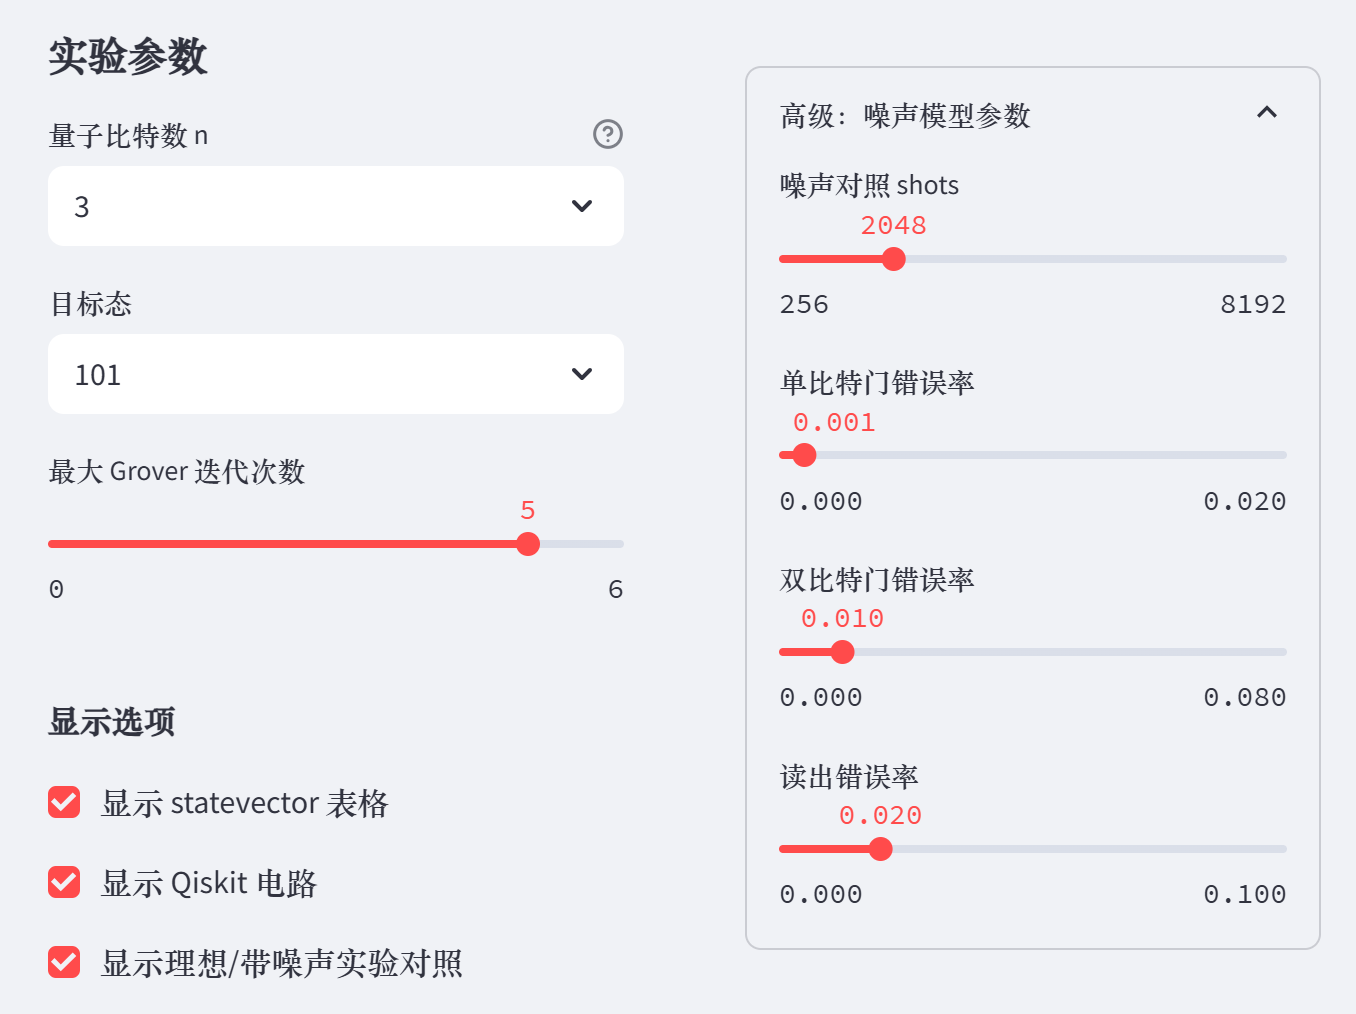
\includegraphics[width=0.95\textwidth]{images/web_crops/sidebar_combined.png}
  }{
    \fbox{\parbox[c][5cm][c]{0.9\textwidth}{\centering 待插入侧边栏参数截图}}
  }
  \caption{Streamlit侧边栏中的实验参数设置}
  \label{fig:web-sidebar}
\end{figure}

\subsection{步进式概率幅与概率展示}

图~\ref{fig:web-step-view}展示了当前步骤的可视化界面。
页面上方给出目标态、总演化步骤数、最高目标态概率和经验最佳迭代次数等摘要信息；
中间区域通过“上一步”“下一步”和滑块选择不同演化步骤；
下方两张柱状图分别显示当前statevector中各计算基态的实数概率幅和测量概率。
目标态使用橙色突出显示。
% Oracle步骤后，目标态概率幅的符号发生翻转，但测量概率保持不变；
% Diffusion步骤后，目标态概率幅被推高，对应的测量概率明显上升。

\begin{figure}[H]
  \centering
  \IfFileExists{images/web_crops/web_step_view.png}{
    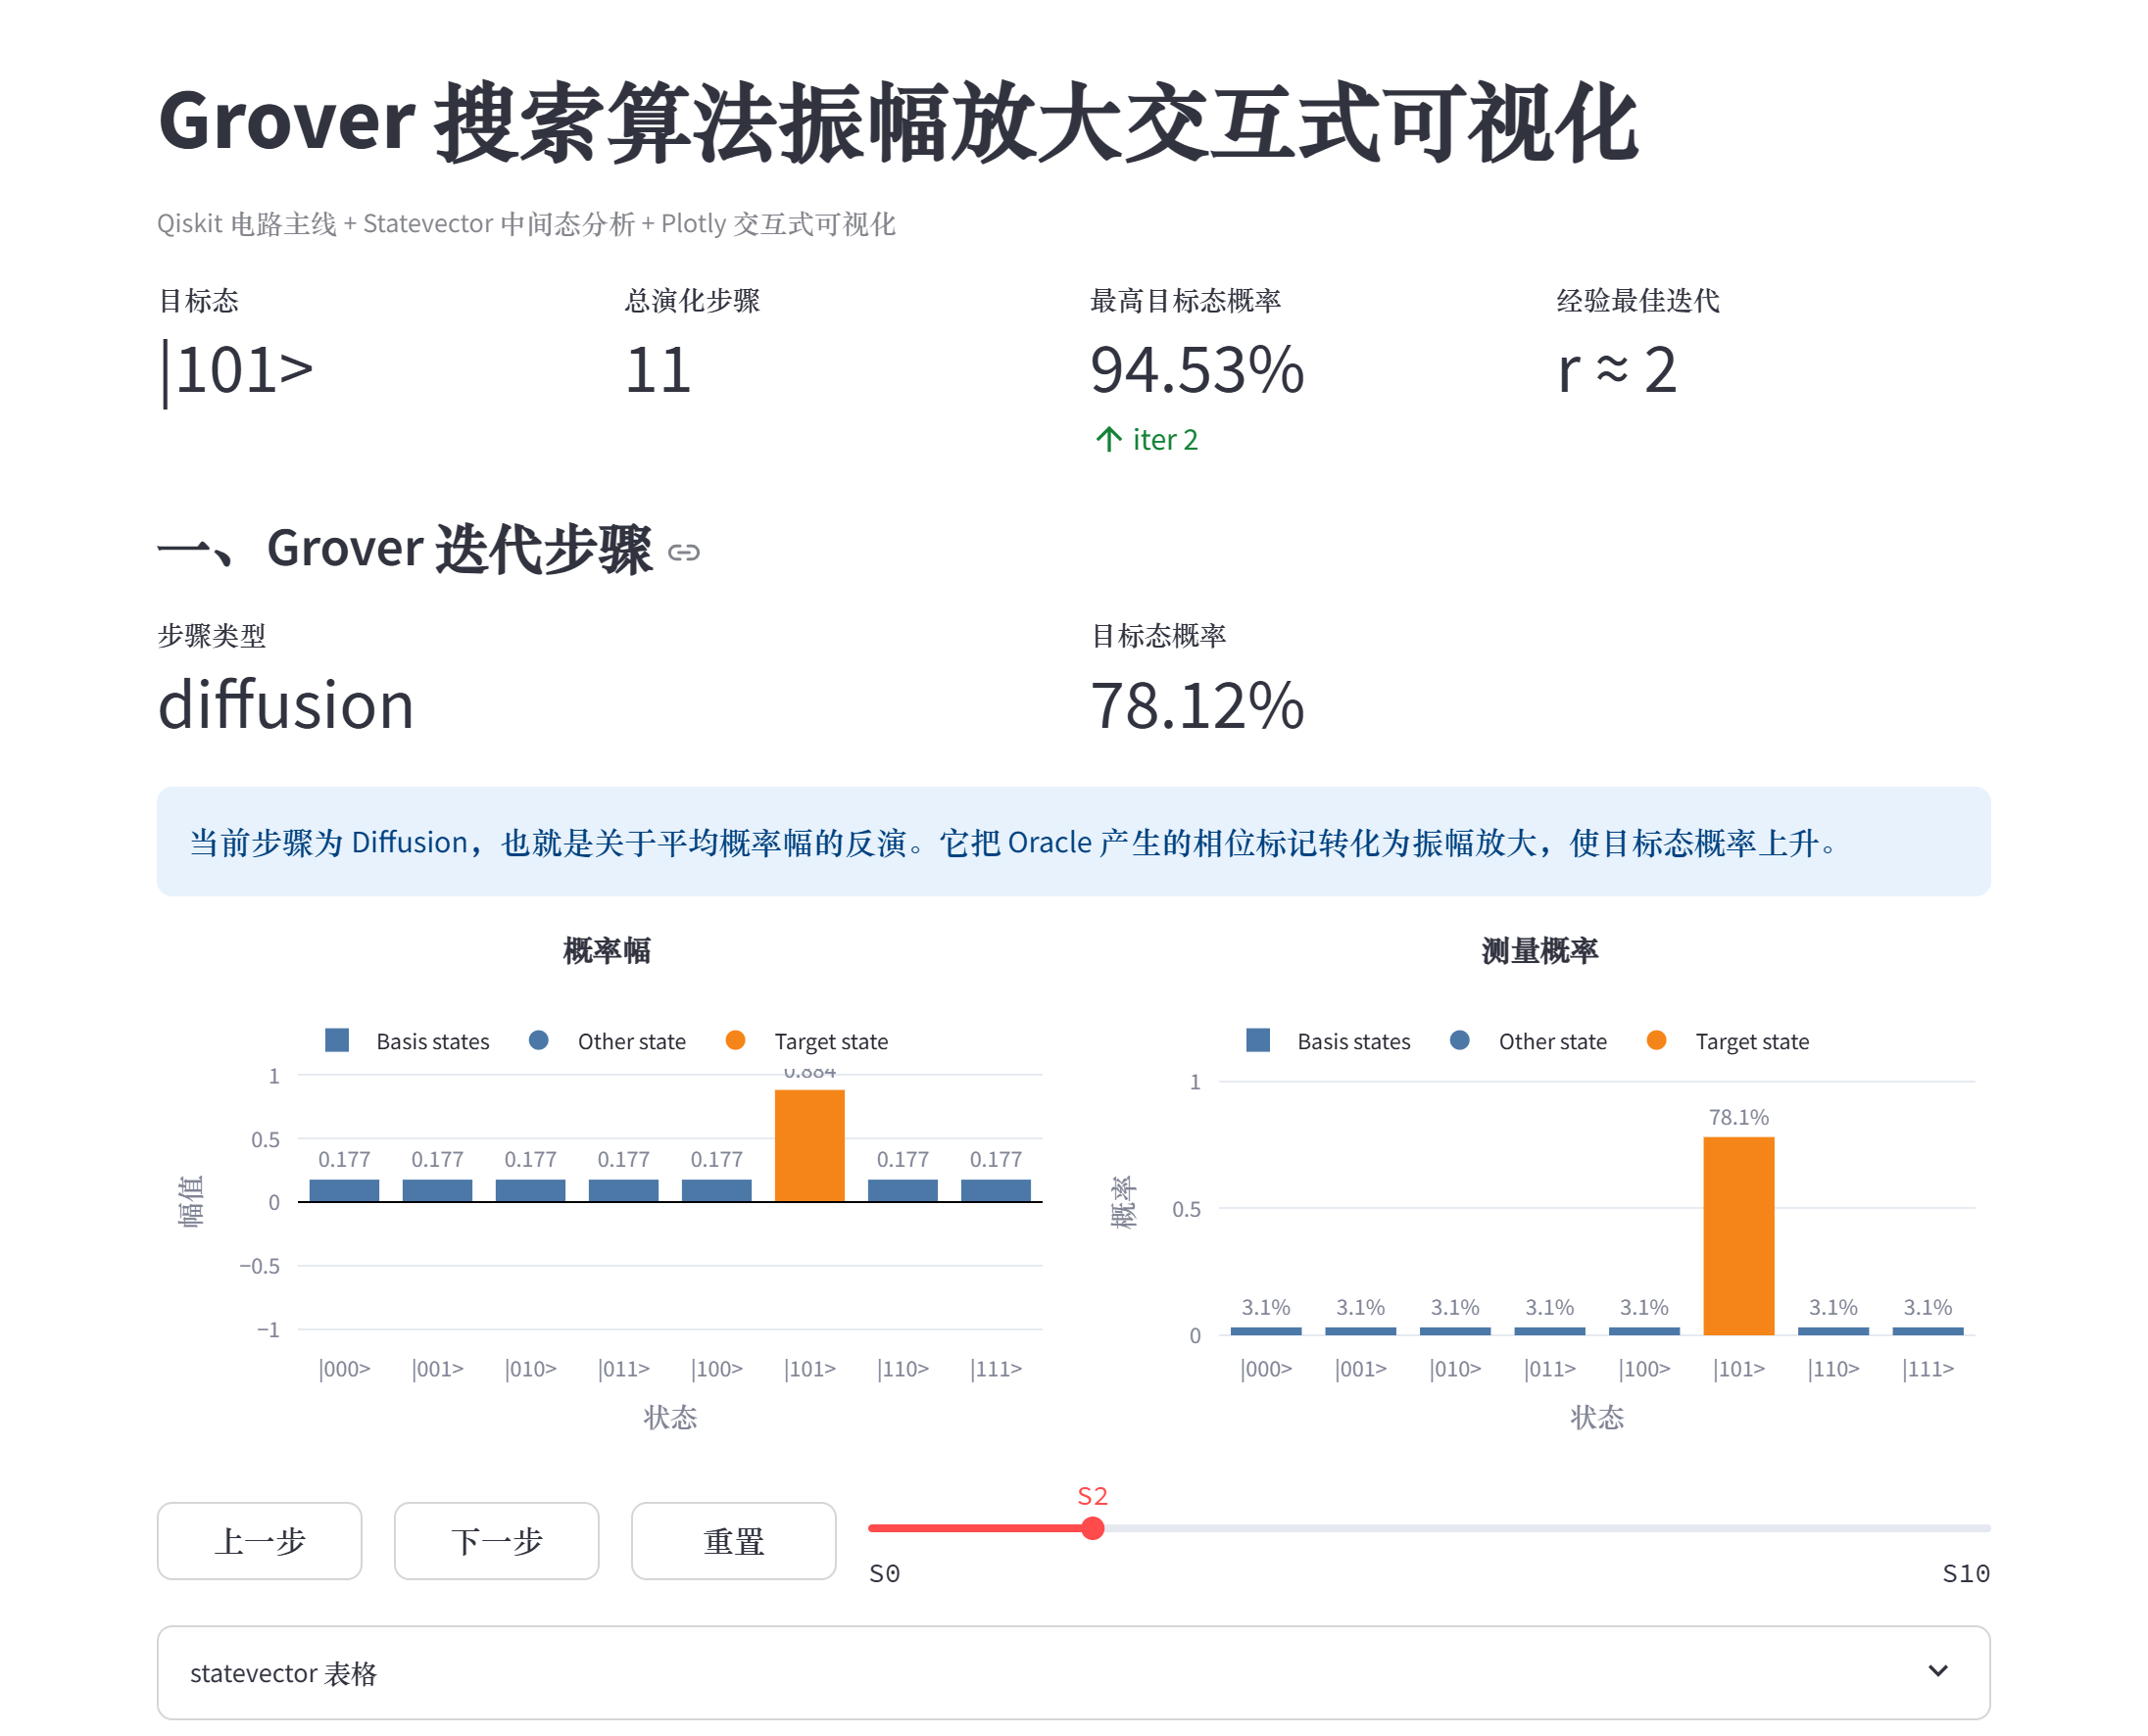
\includegraphics[width=0.95\textwidth]{images/web_crops/web_step_view.png}
  }{
    \fbox{\parbox[c][5cm][c]{0.9\textwidth}{\centering 待插入当前步骤页面截图}}
  }
  \caption{Grover算法当前步骤的概率幅与测量概率可视化界面}
  \label{fig:web-step-view}
\end{figure}

\subsection{目标态概率曲线}

除了单步柱状图外，页面还绘制了目标态概率随完整Grover迭代次数变化的曲线，
如图~\ref{fig:web-target-curve}所示。
该图以完整迭代次数为横轴，以目标态测量概率为纵轴，
用于观察目标态概率在多次Grover迭代中的整体变化趋势。
若侧边栏中最大迭代次数设为5，则曲线会展示\(r=0\)到\(r=5\)的目标态概率；
其中\(r=0\)表示只完成Hadamard初始化，尚未执行Oracle和Diffusion。

对于\(n=3\)、单目标态搜索的示例，第一次完整Grover迭代后目标态概率已经明显升高，
第二次迭代后进一步接近峰值。
该曲线也说明Grover算法并不是迭代次数越多越好，当迭代超过合适次数后，目标态概率会出现回落。
% 因此，页面同时给出经验最佳迭代次数，帮助解释Grover算法中迭代次数选择的重要性。

\begin{figure}[H]
  \centering
  \IfFileExists{images/web_crops/web_target_curve.png}{
    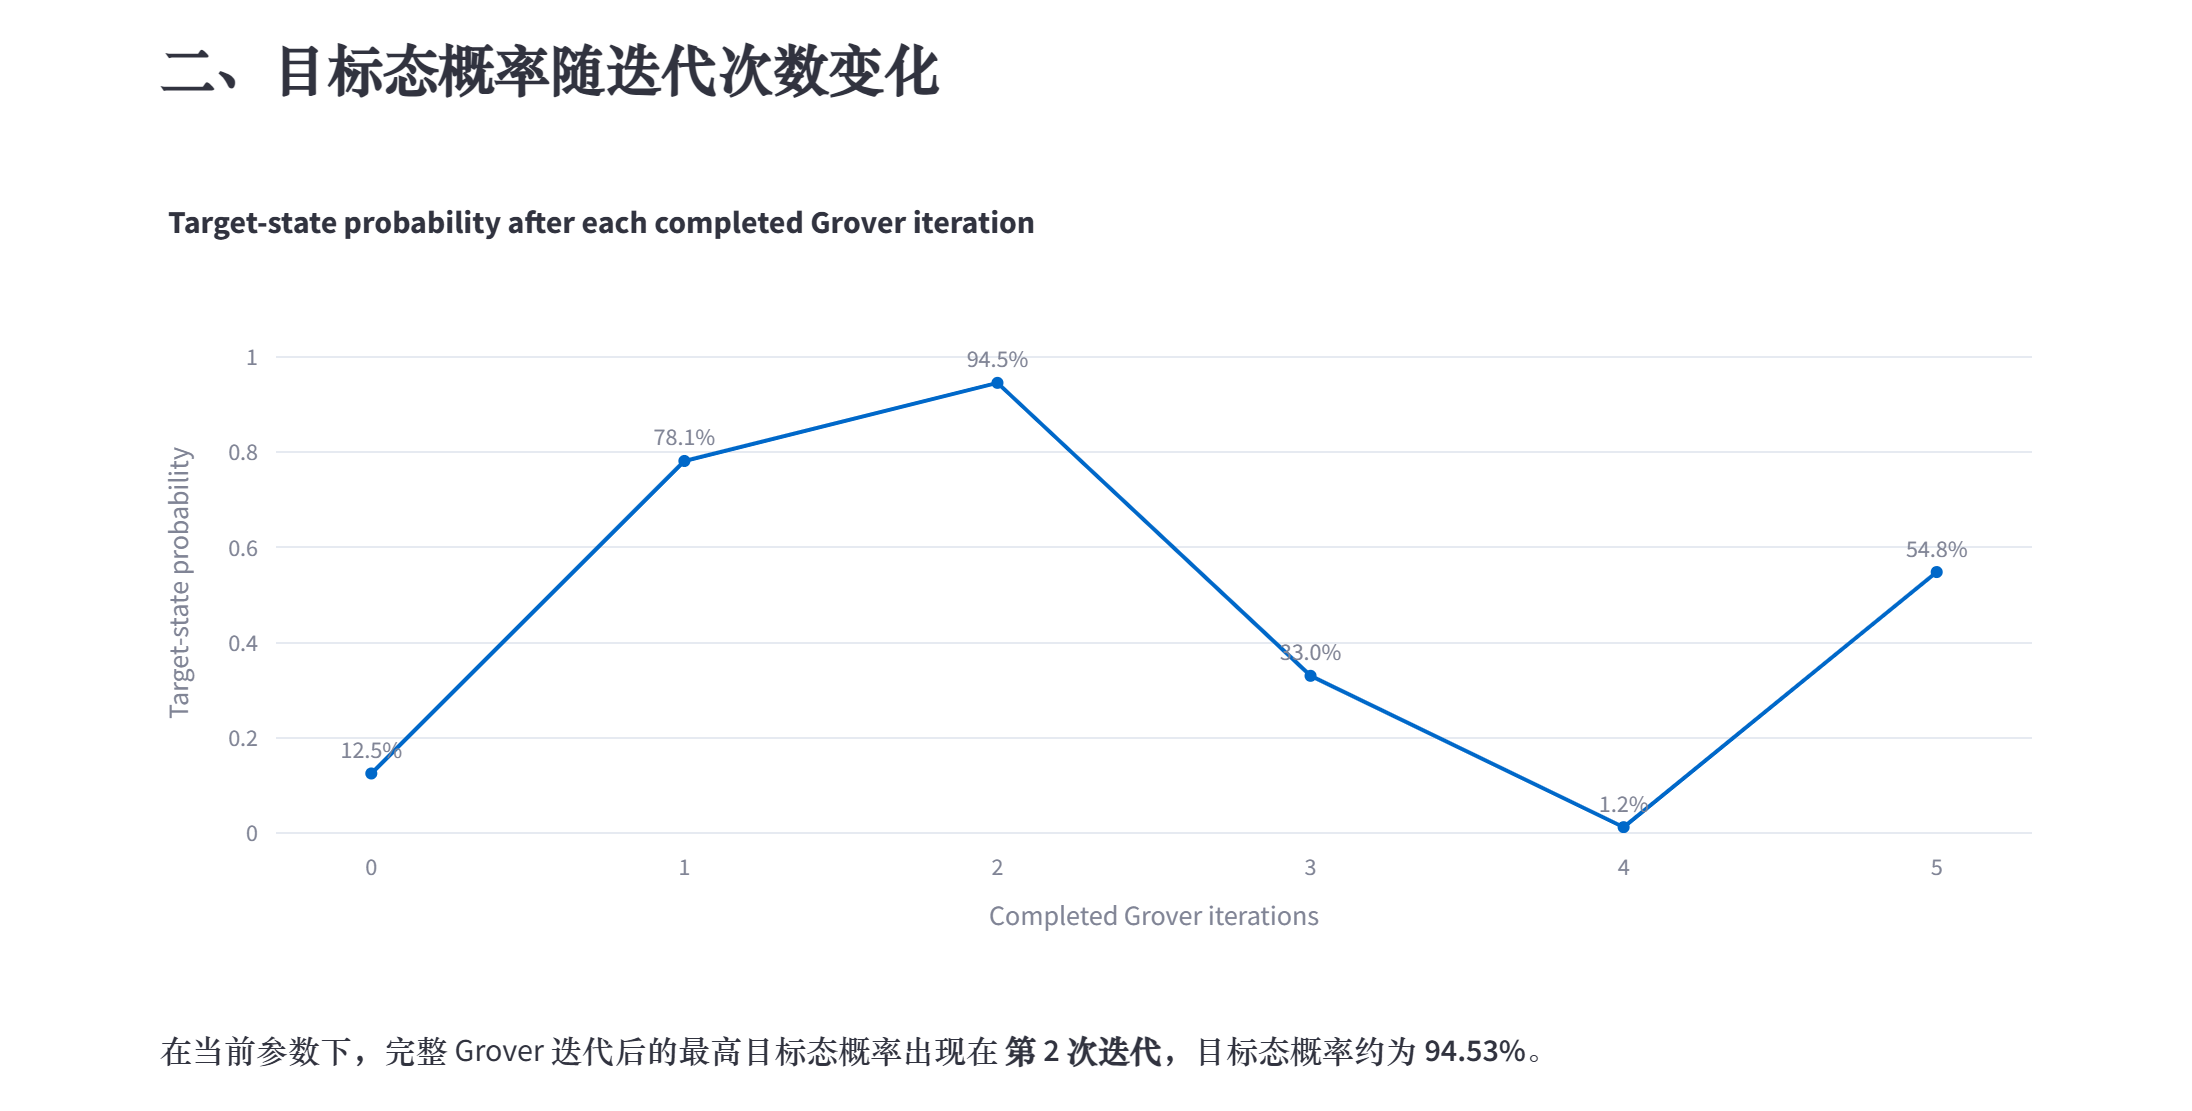
\includegraphics[width=0.88\textwidth]{images/web_crops/web_target_curve.png}
  }{
    \fbox{\parbox[c][5cm][c]{0.9\textwidth}{\centering 待插入目标态概率曲线截图}}
  }
  \caption{目标态概率随完整Grover迭代次数变化的曲线}
  \label{fig:web-target-curve}
\end{figure}

\subsection{Qiskit量子电路结构展示}

图~\ref{fig:web-circuit-view}展示了Qiskit量子电路的交互式操作视图。
该视图将Hadamard初始化、Oracle、Diffusion和测量操作按照电路时间顺序展开，
并保留量子比特线路之间的连接关系。
这一视图能够说明概率幅变化所来自的具体的量子门操作。

在实现上，页面同时提供交互式操作视图、操作表和Qiskit标准电路图三个入口。
交互式操作视图适合观察门操作的顺序和类型，操作表适合检查每一步电路指令，
标准电路图则用于和Qiskit原生绘图结果对照。

\begin{figure}[H]
  \centering
  \IfFileExists{images/web_crops/web_circuit_view.png}{
    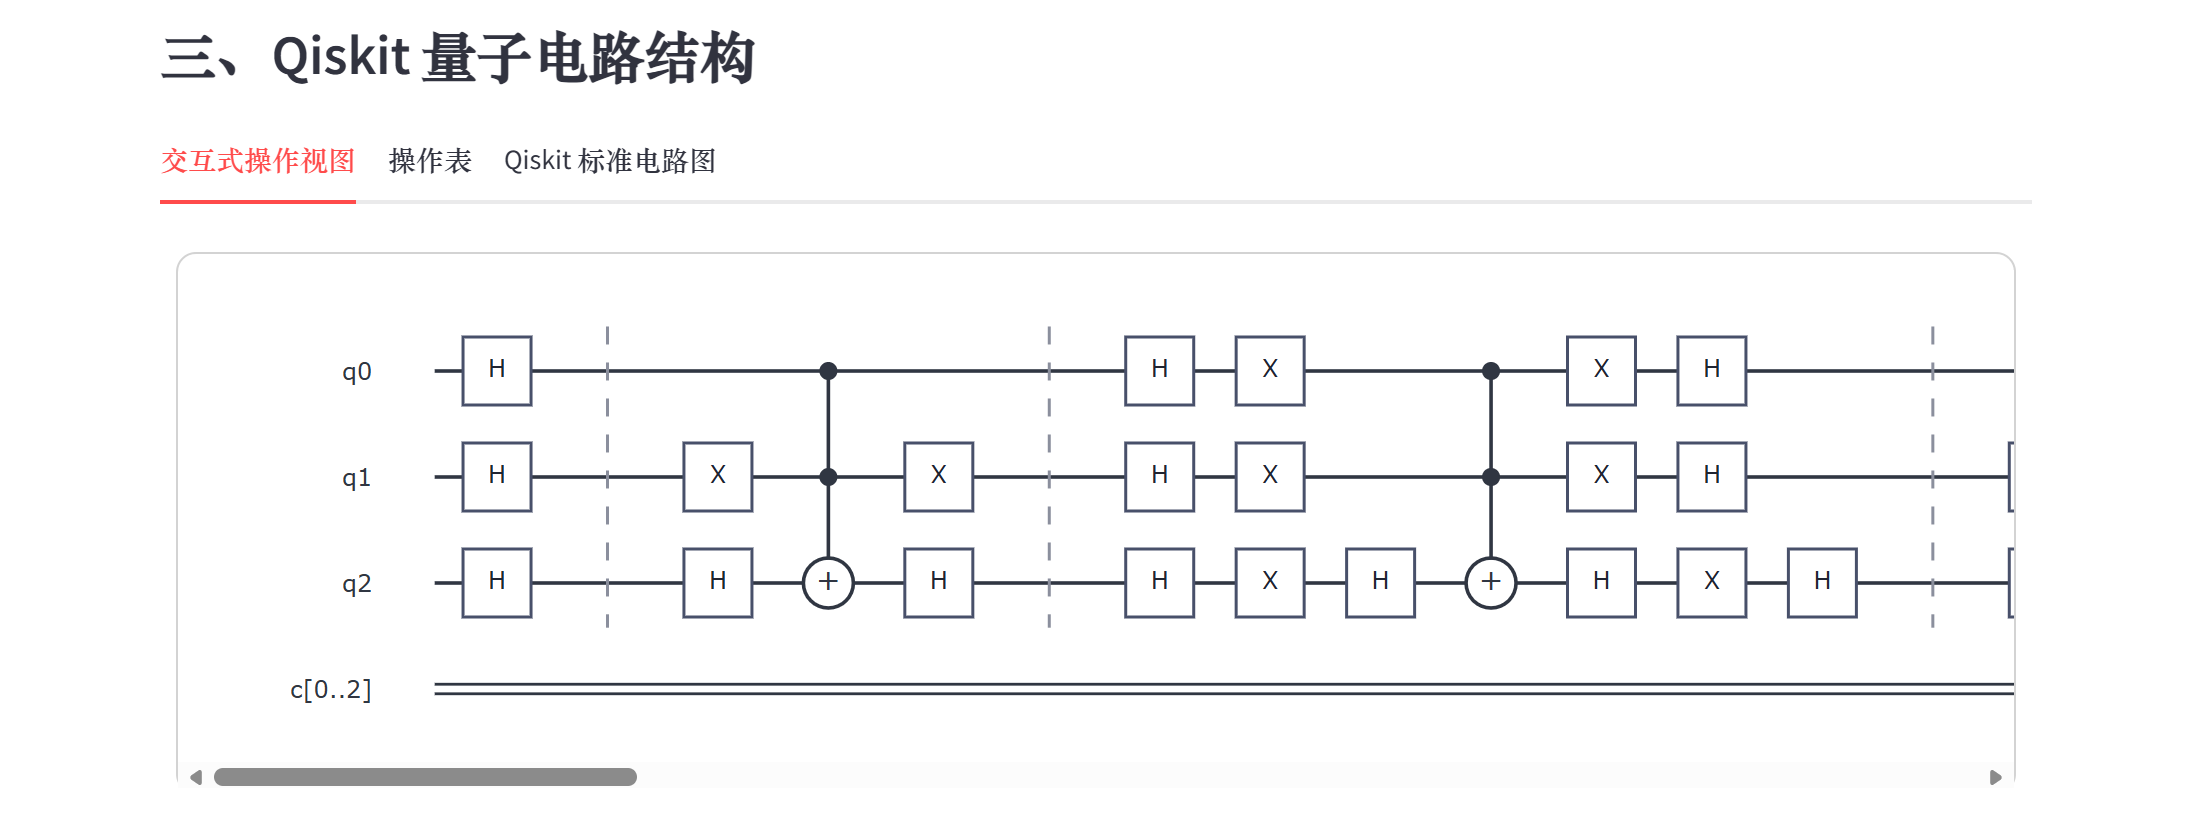
\includegraphics[width=0.95\textwidth]{images/web_crops/web_circuit_view.png}
  }{
    \fbox{\parbox[c][5cm][c]{0.9\textwidth}{\centering 待插入Qiskit电路结构页面截图}}
  }
  \caption{Qiskit量子电路的交互式操作视图}
  \label{fig:web-circuit-view}
\end{figure}

\subsection{理想与带噪声实验对照}

为展示量子电路在带噪声条件下的表现，
页面加入了理想statevector结果与带噪声Aer模拟结果的对照模块，
如图~\ref{fig:web-noise-view}所示。
该模块给出理想目标态概率、带噪声测量频率、目标态损耗、电路深度和CX门数量等摘要指标，
并提供三维分布对照和目标态损耗曲线两个视图。

三维分布对照视图可以在“理想概率分布”“带噪声测量频率”和“理想--带噪声差值”之间切换。
三维分布图说明，当电路深度和多比特门数量增加时，带噪声测量结果会偏离理想概率分布。
目标态损耗曲线则从整体趋势上展示理想概率与带噪声频率之间的差异。

\begin{figure}[H]
  \centering
  \IfFileExists{images/web_crops/web_noise_view.png}{
    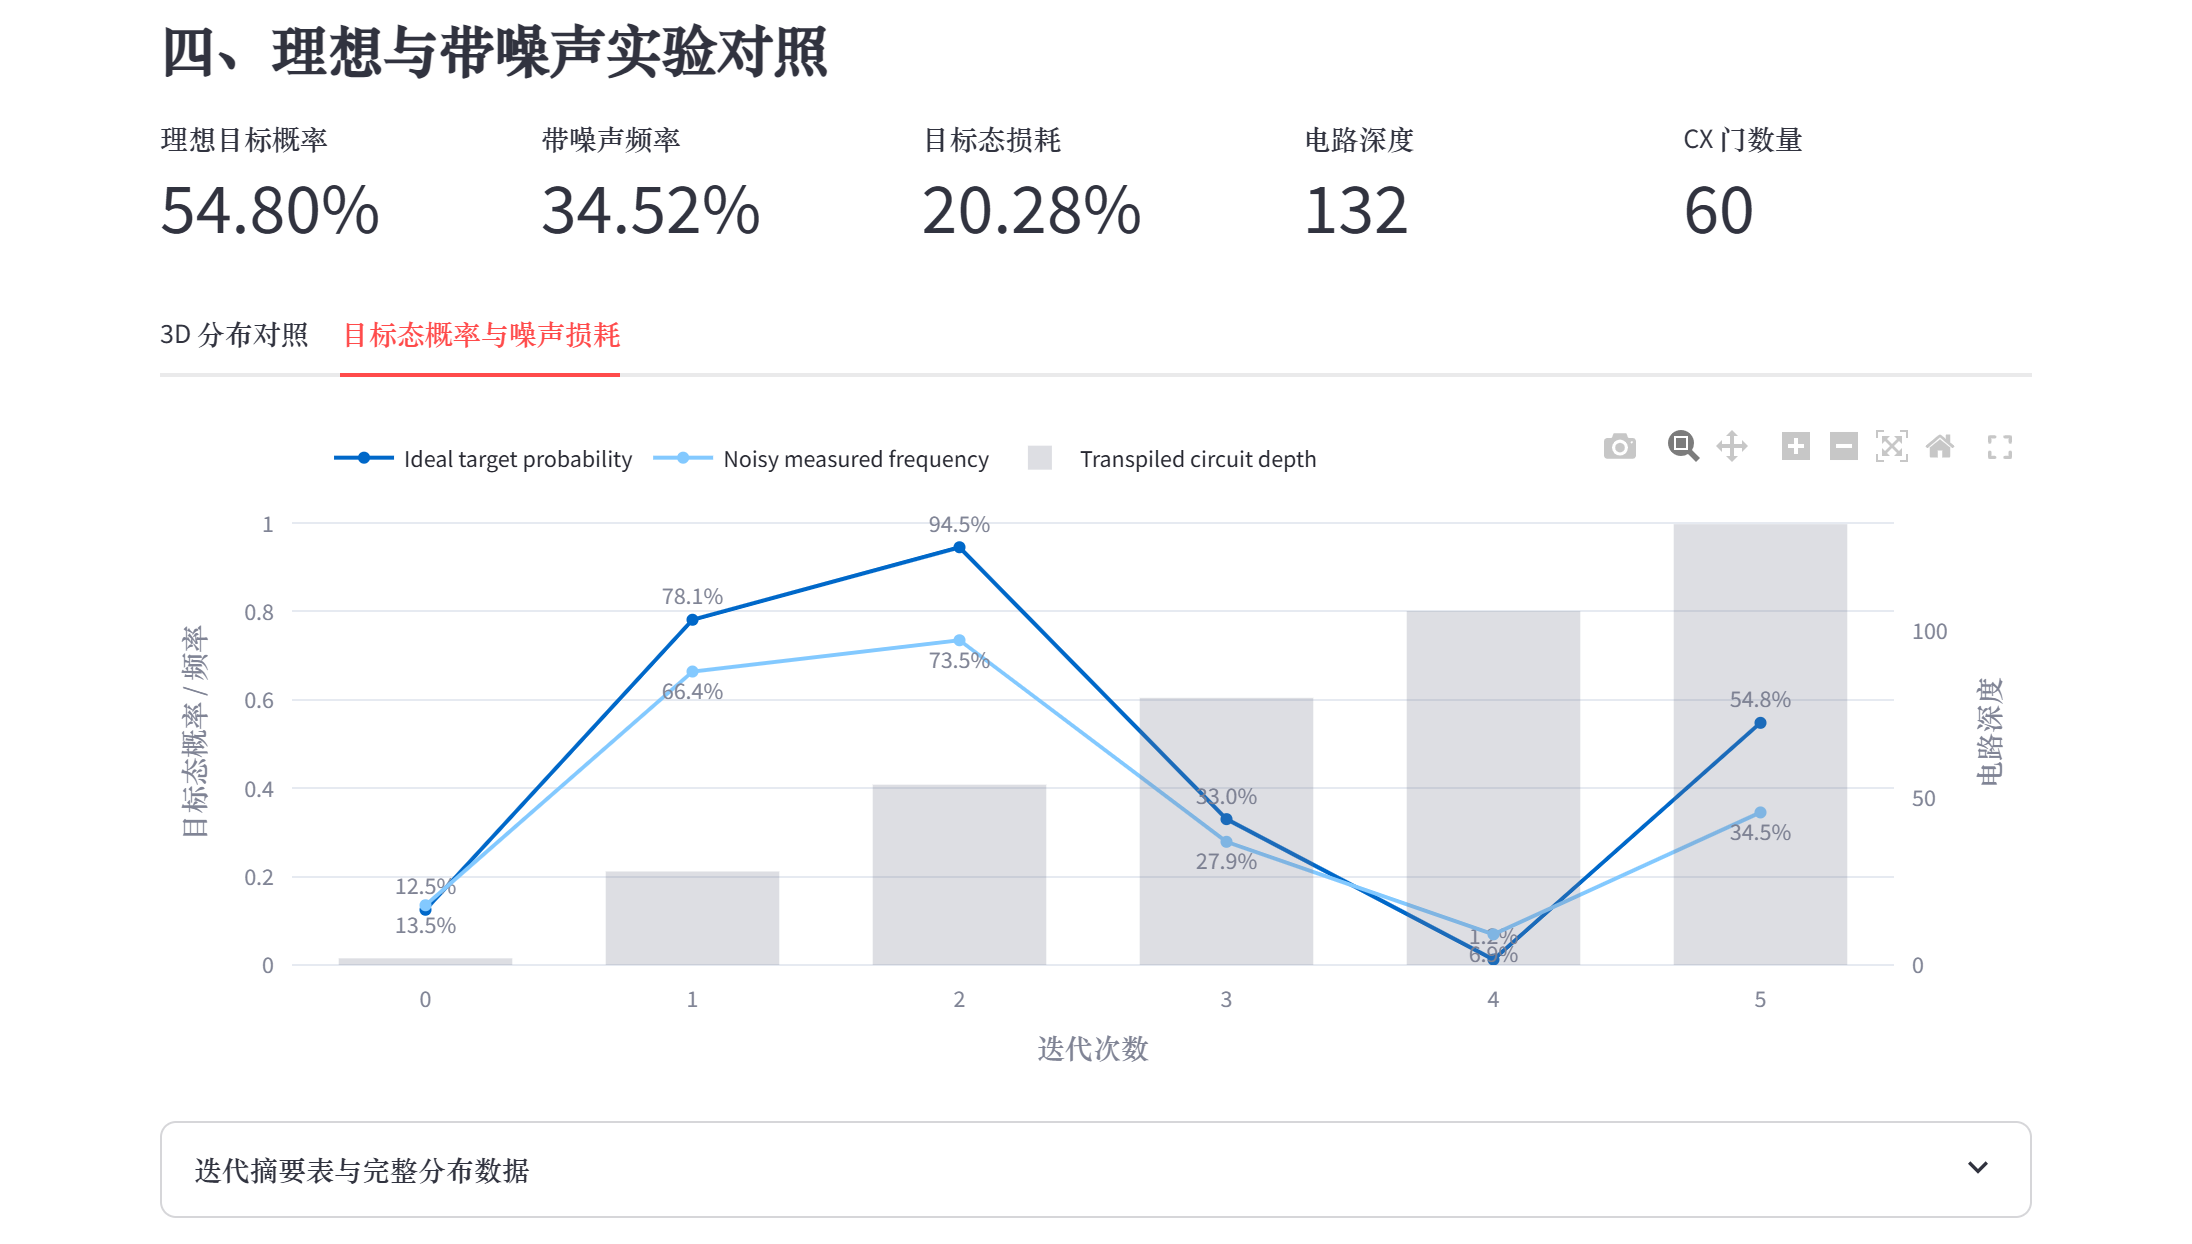
\includegraphics[width=0.95\textwidth]{images/web_crops/web_noise_view.png}
  }{
    \fbox{\parbox[c][5cm][c]{0.9\textwidth}{\centering 待插入理想与带噪声实验对照截图}}
  }
  \caption{理想概率分布与带噪声测量结果的对照视图}
  \label{fig:web-noise-view}
\end{figure}

\subsection{理论解释与错误迭代展示}

图~\ref{fig:web-theory-view}展示了页面中的理论解释区域。
该部分将Grover算法的理论概率公式、模拟结果和过迭代现象放在一起，
用于说明可视化结果与理论模型之间的对应关系。
对于单目标态搜索，目标态概率可以写为
\[
  P_r=\sin^2((2r+1)\theta),
\]
其中\(\sin(\theta)=1/\sqrt{N}\)。
页面根据当前量子比特数和目标态自动计算理论概率，并与程序模拟得到的目标态概率进行对照。

此外，页面还展示了错误迭代或过迭代时目标概率下降的现象，并说明Grover算法的振幅放大的周期性。

\begin{figure}[H]
  \centering
  \IfFileExists{images/web_crops/web_theory_view.png}{
    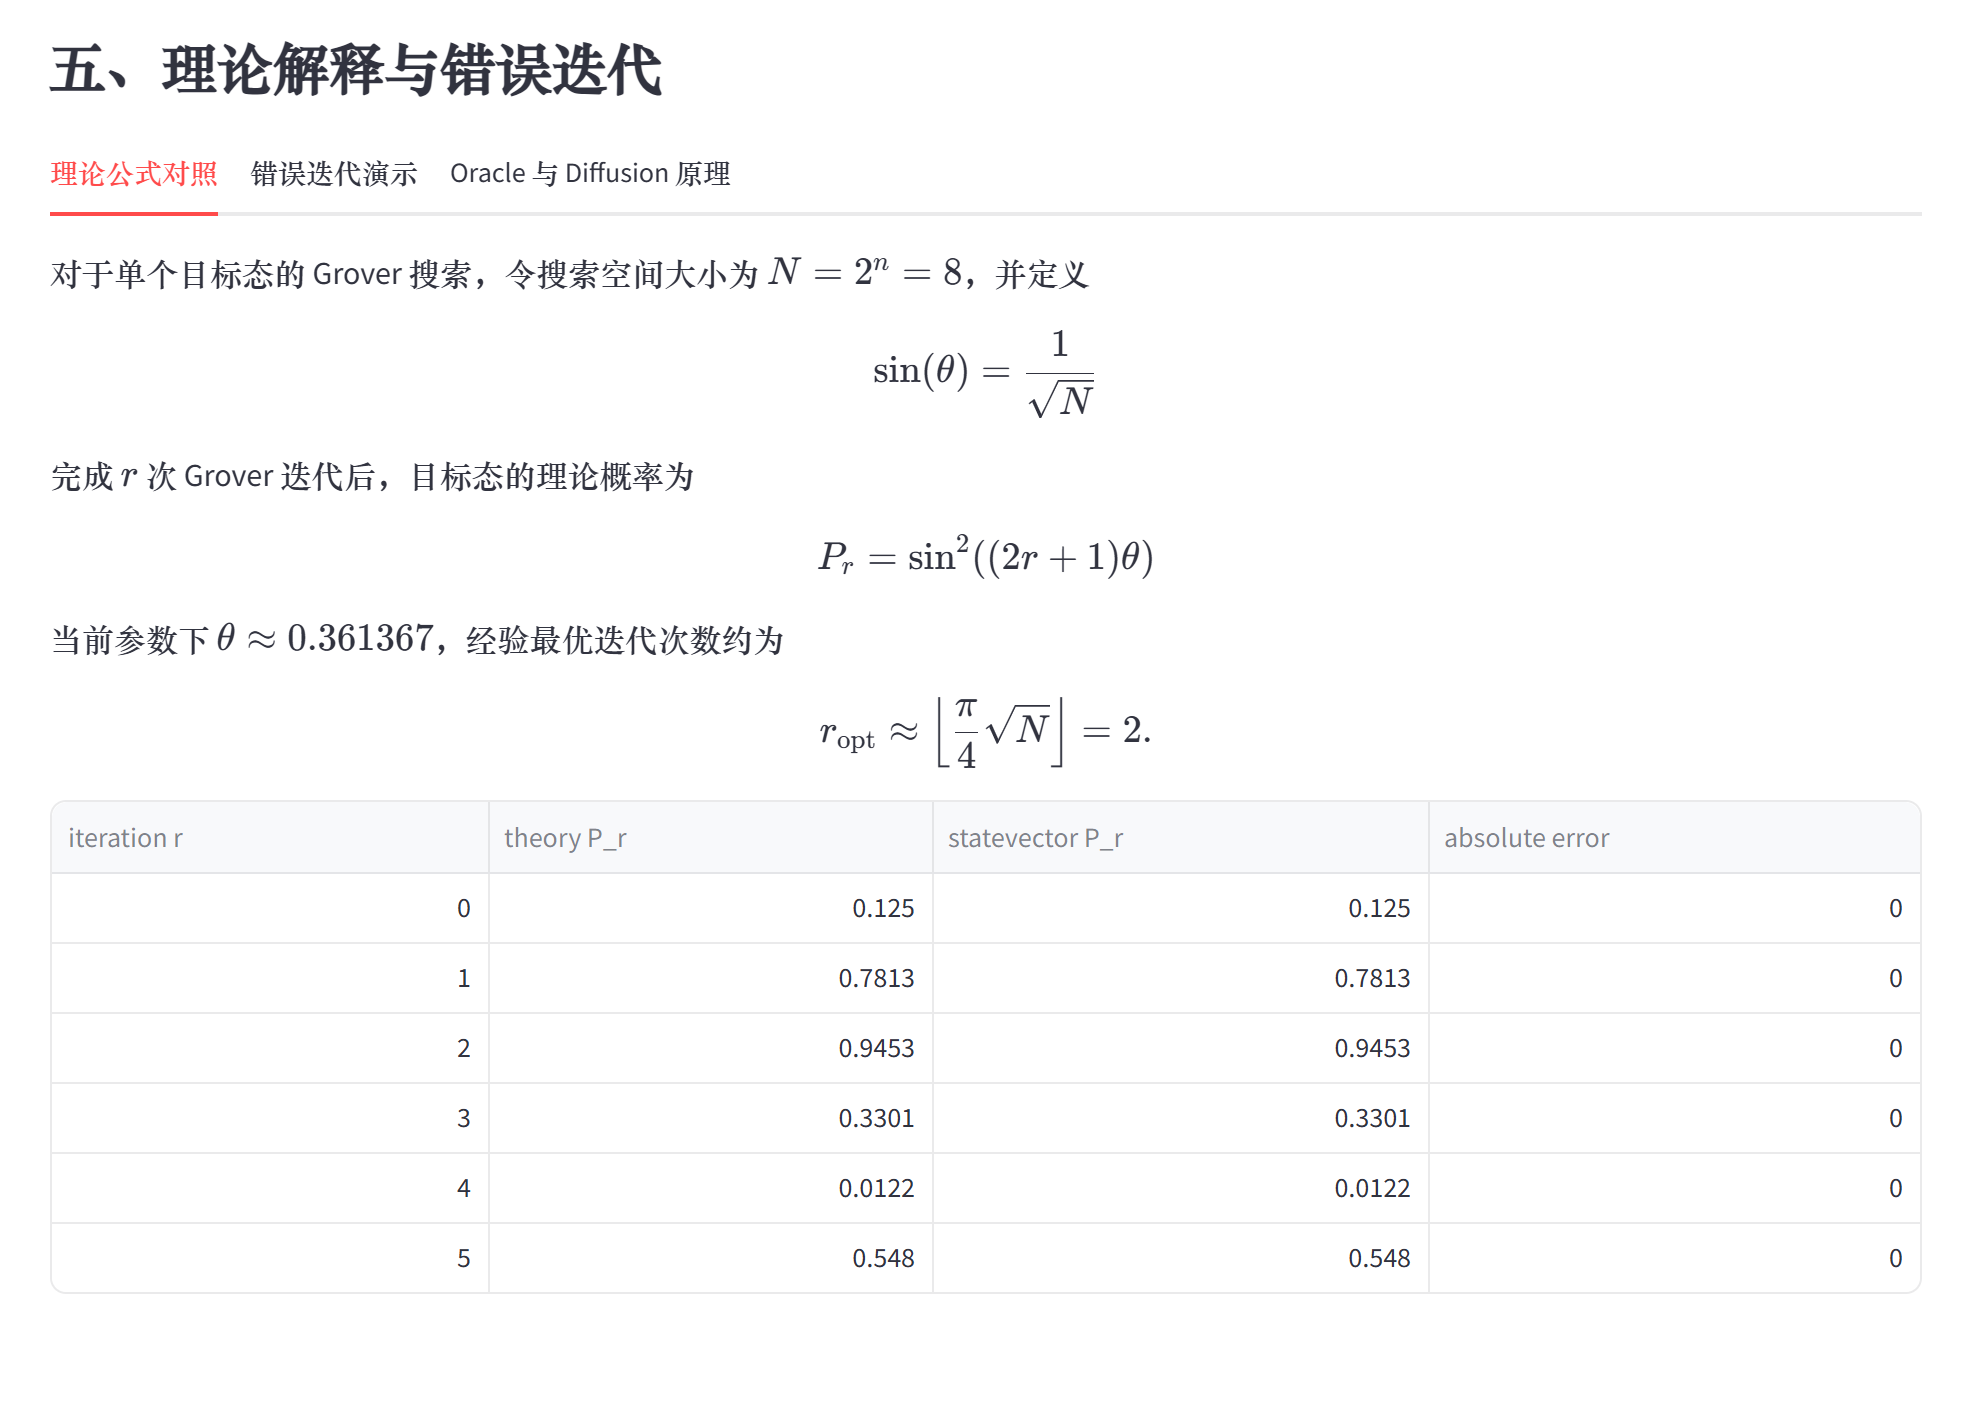
\includegraphics[width=0.95\textwidth]{images/web_crops/web_theory_view.png}
  }{
    \fbox{\parbox[c][5cm][c]{0.9\textwidth}{\centering 待插入理论解释与错误迭代截图}}
  }
  \caption{理论公式、模拟结果与过迭代现象的页面展示}
  \label{fig:web-theory-view}
\end{figure}

\section{运行结果}

\subsection{3量子比特目标态\texorpdfstring{\(|101\rangle\)}{|101>}示例}

选取\(n=3\)、目标态\(|101\rangle\)、迭代次数为2。此时搜索空间大小为\(N=8\)，初始每个基态概率幅为
\[
\frac{1}{\sqrt{8}}\approx 0.353553,
\]
每个基态概率为\(1/8=0.125\)。

\begin{table}[H]
\centering
\caption{\(n=3\)、目标态\(|101\rangle\)时目标态概率幅和概率变化}
\begin{tabular}{llll}
\toprule
步骤 & 操作 & 目标态概率幅 & 目标态概率 \\
\midrule
S0 & Hadamard均匀叠加 & \(+0.353553\) & \(0.125000\) \\
S1 & 第1次Oracle相位翻转 & \(-0.353553\) & \(0.125000\) \\
S2 & 第1次Diffusion均值倒置 & \(+0.883883\) & \(0.781250\) \\
S3 & 第2次Oracle相位翻转 & \(-0.883883\) & \(0.781250\) \\
S4 & 第2次Diffusion均值倒置 & \(+0.972272\) & \(0.945312\) \\
\bottomrule
\end{tabular}
\end{table}

从表中可以看出：
\begin{itemize}
  \item Oracle步骤只改变目标态概率幅符号，不改变目标态概率；
  \item Diffusion步骤把目标态概率幅大幅推高；
  \item 两次完整迭代后，目标态概率达到约\(94.53\%\)；
  \item 如果继续迭代，目标概率会越过最佳点并下降，因此Grover算法需要选择合适的迭代次数。
\end{itemize}

\begin{figure}[H]
  \centering
  \begin{subfigure}[t]{0.48\linewidth}
    \centering
    \IfFileExists{../outputs/figures/00_initial_iter0_amplitude.png}{
      \includegraphics[width=\linewidth]{../outputs/figures/00_initial_iter0_amplitude.png}
    }{
      \fbox{\parbox[c][4.0cm][c]{0.92\linewidth}{\centering 图像文件尚未生成}}
    }
    \caption{初始均匀叠加态的概率幅分布}
  \end{subfigure}
  \hfill
  \begin{subfigure}[t]{0.48\linewidth}
    \centering
    \IfFileExists{../outputs/figures/01_oracle_iter1_amplitude.png}{
      \includegraphics[width=\linewidth]{../outputs/figures/01_oracle_iter1_amplitude.png}
    }{
      \fbox{\parbox[c][4.0cm][c]{0.92\linewidth}{\centering 图像文件尚未生成}}
    }
    \caption{第1次Oracle后目标态概率幅被翻转}
  \end{subfigure}

  \vspace{0.8em}

  \begin{subfigure}[t]{0.48\linewidth}
    \centering
    \IfFileExists{../outputs/figures/02_diffusion_iter1_amplitude.png}{
      \includegraphics[width=\linewidth]{../outputs/figures/02_diffusion_iter1_amplitude.png}
    }{
      \fbox{\parbox[c][4.0cm][c]{0.92\linewidth}{\centering 图像文件尚未生成}}
    }
    \caption{第1次Diffusion后目标态概率幅被放大}
  \end{subfigure}
  \hfill
  \begin{subfigure}[t]{0.48\linewidth}
    \centering
    \IfFileExists{../outputs/figures/03_oracle_iter2_amplitude.png}{
      \includegraphics[width=\linewidth]{../outputs/figures/03_oracle_iter2_amplitude.png}
    }{
      \fbox{\parbox[c][4.0cm][c]{0.92\linewidth}{\centering 图像文件尚未生成}}
    }
    \caption{第2次Oracle后目标态概率幅再次翻转}
  \end{subfigure}

  \vspace{0.8em}

  \begin{subfigure}[t]{0.48\linewidth}
    \centering
    \IfFileExists{../outputs/figures/04_diffusion_iter2_amplitude.png}{
      \includegraphics[width=\linewidth]{../outputs/figures/04_diffusion_iter2_amplitude.png}
    }{
      \fbox{\parbox[c][4.0cm][c]{0.92\linewidth}{\centering 图像文件尚未生成}}
    }
    \caption{第2次Diffusion后目标态概率幅继续增大}
  \end{subfigure}
  \hfill
  \begin{subfigure}[t]{0.48\linewidth}
    \centering
    \IfFileExists{../outputs/figures/target_probability_curve.png}{
      \includegraphics[width=\linewidth]{../outputs/figures/target_probability_curve.png}
    }{
      \fbox{\parbox[c][4.0cm][c]{0.92\linewidth}{\centering 图像文件尚未生成}}
    }
    \caption{目标态概率随完整Grover迭代次数变化}
  \end{subfigure}
  \caption{\(n=3\)、目标态\(|101\rangle\)时两次Grover迭代中的概率幅变化}
\end{figure}

\subsection{与理论结果对照}

对\(N=8\)，有
\[
\theta=\arcsin\left(\frac{1}{\sqrt{8}}\right).
\]
代入理论公式：
\[
P_1=\sin^2(3\theta)=0.78125,
\]
\[
P_2=\sin^2(5\theta)=0.9453125.
\]
这与程序中statevector计算得到的结果一致，说明电路构造和图表数据提取是正确的。

\subsection{2量子比特情况}

当\(n=2\)时，\(N=4\)。单目标Grover搜索在一次完整迭代后即可把目标态概率提升到1。
当\(n=3\)时，目标态概率在多次迭代中先上升后回落，程序通过目标态概率曲线记录这一过迭代现象。

\section{问题与改进}

\subsection{已完成的功能}

\begin{enumerate}
  \item \textbf{保存中间态。} 项目在每次Oracle和Diffusion后保存statevector，形成完整的步骤序列。
  \item \textbf{同时计算概率幅和概率。} 概率幅图给出Oracle后的符号翻转，概率图给出Diffusion后的测量概率提升。
  \item \textbf{生成3D步进图。} 3D图把“基态--步骤--概率”放在同一个坐标系中，记录目标态概率柱随步骤升高的过程。
  \item \textbf{提供交互参数。} 用户可以切换量子比特数、目标态、迭代次数，并通过滑块选择当前步骤。
  \item \textbf{保留量子电路信息。} 除图表外，界面还显示Qiskit标准电路图和交互式操作表，使每一步状态变化对应到具体量子门。
\end{enumerate}

\subsection{不足与改进方向}

本项目按照课程项目要求支持2到3个量子比特。若扩展到更多量子比特，柱状图数量会迅速增加，3D图也会变得拥挤，需要改用筛选、聚类或只突出目标态和若干代表性非目标态的方式。

另一方面，当前噪声模型只是简化的depolarizing noise和readout noise，不代表真实量子硬件的校准噪声。后续可以接入真实后端参数，或加入多目标Grover搜索。

\section{结论}

本项目完成了一个基于Qiskit、Streamlit和Plotly的Grover搜索算法振幅放大可视化系统。系统支持2到3个量子比特，能够选择任意目标态，并在Hadamard初始化、Oracle相位翻转和Diffusion均值倒置后保存并展示中间statevector。

通过\(n=3\)、目标态\(|101\rangle\)的实验可以看到，Oracle只是将目标态概率幅变为负值，目标态概率并未立即增加；随后Diffusion通过关于平均概率幅的反演，把相位标记转化为振幅放大，使目标态概率从\(12.5\%\)逐步提升到\(78.125\%\)和\(94.53125\%\)。这一结果与Grover算法理论公式一致。

因此，本项目较好地完成了课程选题要求：利用柱状图和3D步进图展示Grover搜索算法中目标态概率幅被逐步放大的过程，并通过交互界面降低了抽象量子态演化的理解难度。

\begin{thebibliography}{9}
    \bibitem{grover1996}
    L. K. Grover, ``A fast quantum mechanical algorithm for database search,'' Proceedings of the 28th Annual ACM Symposium on Theory of Computing, 1996.

    \bibitem{qiskit}
    Qiskit Documentation, \url{https://docs.quantum.ibm.com/}

    \bibitem{streamlit}
    Streamlit Documentation, \url{https://docs.streamlit.io/}

    \bibitem{plotly}
    Plotly Python Documentation, \url{https://plotly.com/python/}
\end{thebibliography}


\end{document}
